

\tikzset{every picture/.style={line width=0.75pt}} %set default line width to 0.75pt        

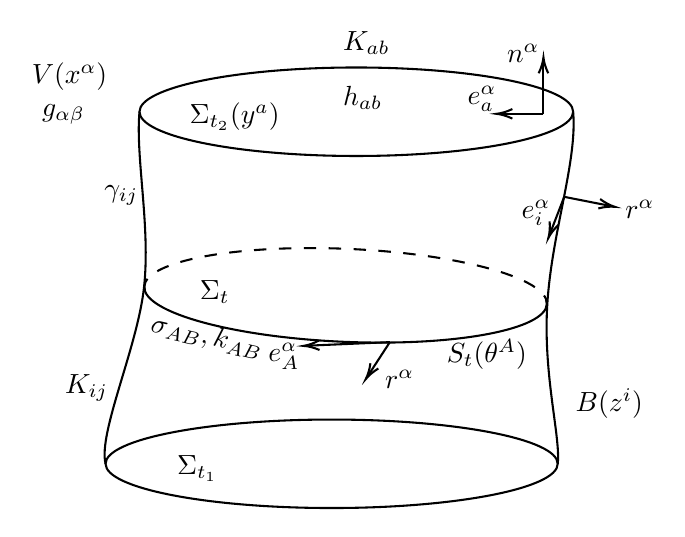
\begin{tikzpicture}[x=0.75pt,y=0.75pt,yscale=-1,xscale=1]
	%uncomment if require: \path (0,240); %set diagram left start at 0, and has height of 240
	
	%Curve Lines [id:da786565528514253] 
	\draw    (224.37,43) .. controls (222.37,64.68) and (229.72,98.24) .. (226.58,127.35) .. controls (223.45,156.47) and (204.37,197.68) .. (208.02,212.62) ;
	%Curve Lines [id:da21360769104042077] 
	\draw    (433.3,43) .. controls (435.37,66.68) and (423.29,100.08) .. (420.92,134.69) .. controls (418.55,169.29) and (427.37,199.68) .. (425.87,212.62) ;
	%Shape: Ellipse [id:dp6546353513348666] 
	\draw   (224.37,43) .. controls (224.37,31.23) and (271.14,21.68) .. (328.83,21.68) .. controls (386.53,21.68) and (433.3,31.23) .. (433.3,43) .. controls (433.3,54.77) and (386.53,64.32) .. (328.83,64.32) .. controls (271.14,64.32) and (224.37,54.77) .. (224.37,43) -- cycle ;
	%Shape: Ellipse [id:dp6835416852337497] 
	\draw   (208.02,212.62) .. controls (208.02,200.85) and (256.79,191.3) .. (316.94,191.3) .. controls (377.1,191.3) and (425.87,200.85) .. (425.87,212.62) .. controls (425.87,224.39) and (377.1,233.93) .. (316.94,233.93) .. controls (256.79,233.93) and (208.02,224.39) .. (208.02,212.62) -- cycle ;
	%Shape: Arc [id:dp06149673780052711] 
	\draw  [draw opacity=0] (420.41,133.77) .. controls (420.6,134.38) and (420.68,135) .. (420.66,135.62) .. controls (420.13,147.98) and (376.27,156.14) .. (322.7,153.84) .. controls (269.14,151.53) and (226.14,139.65) .. (226.67,127.29) .. controls (226.68,127.04) and (226.71,126.8) .. (226.76,126.56) -- (323.67,131.45) -- cycle ; \draw   (420.41,133.77) .. controls (420.6,134.38) and (420.68,135) .. (420.66,135.62) .. controls (420.13,147.98) and (376.27,156.14) .. (322.7,153.84) .. controls (269.14,151.53) and (226.14,139.65) .. (226.67,127.29) .. controls (226.68,127.04) and (226.71,126.8) .. (226.76,126.56) ;
	%Shape: Arc [id:dp8928990689301937] 
	\draw  [draw opacity=0][dash pattern={on 4.5pt off 4.5pt}] (226.92,129.14) .. controls (226.73,128.52) and (226.65,127.91) .. (226.67,127.29) .. controls (227.2,114.93) and (271.06,106.77) .. (324.63,109.07) .. controls (378.19,111.37) and (421.19,123.26) .. (420.66,135.62) .. controls (420.65,135.86) and (420.62,136.11) .. (420.58,136.35) -- (323.67,131.45) -- cycle ; \draw  [dash pattern={on 4.5pt off 4.5pt}] (226.92,129.14) .. controls (226.73,128.52) and (226.65,127.91) .. (226.67,127.29) .. controls (227.2,114.93) and (271.06,106.77) .. (324.63,109.07) .. controls (378.19,111.37) and (421.19,123.26) .. (420.66,135.62) .. controls (420.65,135.86) and (420.62,136.11) .. (420.58,136.35) ;
	%Straight Lines [id:da6366675243909421] 
	\draw    (419,44) -- (419,18.81) ;
	\draw [shift={(419,16.81)}, rotate = 450] [color={rgb, 255:red, 0; green, 0; blue, 0 }  ][line width=0.75]    (7.65,-2.3) .. controls (4.86,-0.97) and (2.31,-0.21) .. (0,0) .. controls (2.31,0.21) and (4.86,0.98) .. (7.65,2.3)   ;
	%Straight Lines [id:da950798834233882] 
	\draw    (419,44) -- (398.37,44) ;
	\draw [shift={(396.37,44)}, rotate = 360] [color={rgb, 255:red, 0; green, 0; blue, 0 }  ][line width=0.75]    (7.65,-2.3) .. controls (4.86,-0.97) and (2.31,-0.21) .. (0,0) .. controls (2.31,0.21) and (4.86,0.98) .. (7.65,2.3)   ;
	%Straight Lines [id:da9599405099391465] 
	\draw    (345,154) -- (334.46,170.18) ;
	\draw [shift={(333.37,171.85)}, rotate = 303.09000000000003] [color={rgb, 255:red, 0; green, 0; blue, 0 }  ][line width=0.75]    (7.65,-2.3) .. controls (4.86,-0.97) and (2.31,-0.21) .. (0,0) .. controls (2.31,0.21) and (4.86,0.98) .. (7.65,2.3)   ;
	%Straight Lines [id:da28714016794972896] 
	\draw    (345,154) -- (305.36,155.72) ;
	\draw [shift={(303.37,155.81)}, rotate = 357.52] [color={rgb, 255:red, 0; green, 0; blue, 0 }  ][line width=0.75]    (7.65,-2.3) .. controls (4.86,-0.97) and (2.31,-0.21) .. (0,0) .. controls (2.31,0.21) and (4.86,0.98) .. (7.65,2.3)   ;
	%Straight Lines [id:da5740479448727278] 
	\draw    (429,84) -- (451.4,88.42) ;
	\draw [shift={(453.37,88.81)}, rotate = 191.16] [color={rgb, 255:red, 0; green, 0; blue, 0 }  ][line width=0.75]    (7.65,-2.3) .. controls (4.86,-0.97) and (2.31,-0.21) .. (0,0) .. controls (2.31,0.21) and (4.86,0.98) .. (7.65,2.3)   ;
	%Straight Lines [id:da23796795663259163] 
	\draw    (429,84) -- (422.08,101.94) ;
	\draw [shift={(421.37,103.81)}, rotate = 291.08] [color={rgb, 255:red, 0; green, 0; blue, 0 }  ][line width=0.75]    (7.65,-2.3) .. controls (4.86,-0.97) and (2.31,-0.21) .. (0,0) .. controls (2.31,0.21) and (4.86,0.98) .. (7.65,2.3)   ;
	
	
	% Text Node
	\draw (241,207) node [anchor=north west][inner sep=0.75pt]    {$\Sigma _{t_{1}}$};
	% Text Node
	\draw (247,37) node [anchor=north west][inner sep=0.75pt]    {$\Sigma _{t_{2}} (y^{a} )$};
	% Text Node
	\draw (252,123) node [anchor=north west][inner sep=0.75pt]    {$\Sigma _{t}$};
	% Text Node
	\draw (371,151) node [anchor=north west][inner sep=0.75pt]    {$S_{t} (\theta ^{A} )$};
	% Text Node
	\draw (433,175) node [anchor=north west][inner sep=0.75pt]    {$\mathscr{B} (z^{i} )$};
	% Text Node
	\draw (171,18) node [anchor=north west][inner sep=0.75pt]    {$\mathscr{V} (x^{\alpha } )$};
	% Text Node
	\draw (400,9) node [anchor=north west][inner sep=0.75pt]    {$n^{\alpha }$};
	% Text Node
	\draw (381,29) node [anchor=north west][inner sep=0.75pt]    {$e_{a}^{\alpha }$};
	% Text Node
	\draw (321,29) node [anchor=north west][inner sep=0.75pt]    {$h_{ab}$};
	% Text Node
	\draw (321,3) node [anchor=north west][inner sep=0.75pt]    {$K_{ab}$};
	% Text Node
	\draw (341.18,165.93) node [anchor=north west][inner sep=0.75pt]    {$r^{\alpha }$};
	% Text Node
	\draw (285,153) node [anchor=north west][inner sep=0.75pt]    {$e_{A}^{\alpha }$};
	% Text Node
	\draw (230.41,137.97) node [anchor=north west][inner sep=0.75pt]  [rotate=-13.09]  {$\sigma _{AB} ,k_{AB}$};
	% Text Node
	\draw (457,84) node [anchor=north west][inner sep=0.75pt]    {$r^{\alpha }$};
	% Text Node
	\draw (407,84) node [anchor=north west][inner sep=0.75pt]    {$e_{i}^{\alpha }$};
	% Text Node
	\draw (206,77) node [anchor=north west][inner sep=0.75pt]    {$\gamma _{ij}$};
	% Text Node
	\draw (187,168) node [anchor=north west][inner sep=0.75pt]    {$\mathscr{K}_{ij}$};
	% Text Node
	\draw (176,38) node [anchor=north west][inner sep=0.75pt]    {$g_{\alpha \beta }$};
	
	
\end{tikzpicture}